\subsection{Local Histogram Processing}

Indtil videre har vi brugt \textit{global histogram processing} til at behandle billederne. Figur~\ref{fig:local-equalization} viser hvordan man med local eq, kan finde detaljer som den globale ikke kunne trække ud.

\begin{figure}[H]
	\centering
	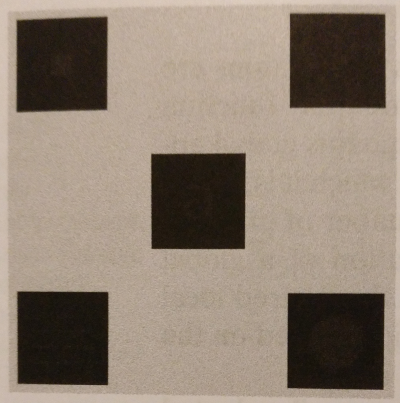
\includegraphics[width=0.3\linewidth]{figs/spm01/original} \hfill
	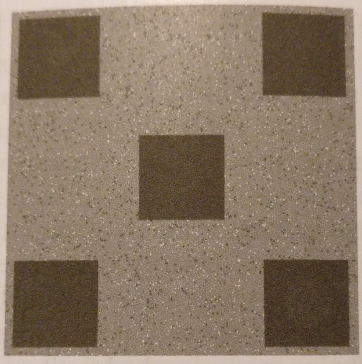
\includegraphics[width=0.3\linewidth]{figs/spm01/global-eq}\hfill
	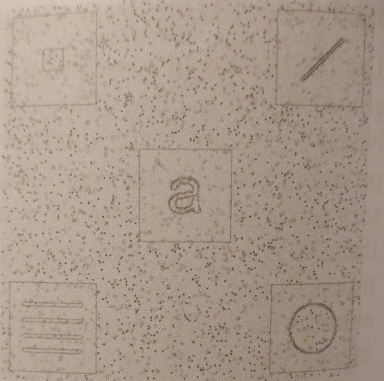
\includegraphics[width=0.3\linewidth]{figs/spm01/local-eq}
	
	\caption{Fra venstre: Det originale billede, billede efter global equalization, efter local. Lavet med \textit{neighborhood size} af 3 x 3.}
	\label{fig:local-equalization}
\end{figure}
